\documentclass[10pt,twoside,openright]{memoir}
\usepackage[paperwidth=4.25in, paperheight=6.875in,bindingoffset=.75in]{geometry}
\usepackage[utf8]{inputenc} % If utf8 encoding                                  
\usepackage[T1]{fontenc}    %                                                   
\usepackage[english]{babel} % English please                                    
\usepackage[final]{microtype} % Less badboxes 
\usepackage{tgpagella}
\usepackage{caption}
\usepackage{graphicx}
\usepackage{rotating}

\makeevenhead{headings}%
    {\thepage}{}{}
\makeoddhead{headings}%
    {}{}{\thepage}

\makeatletter
\def\maketitle{%
  \null
  \thispagestyle{empty}%
  \vfill
  \begin{center}\leavevmode
    \normalfont
    {\LARGE\raggedleft \@author\par}%
    \hrulefill\par
    {\huge\raggedright \@title\par}%
    \vskip 1cm
%    {\Large \@date\par}%
  \end{center}%
  \vfill
  \null
  \cleardoublepage
  }
\makeatother

\author{Tao Lin}
\author{Tao Lin}
\title{North American Hamsters}
\date{}










%%% BEGIN DOCUMENT

\begin{document}

\OnehalfSpacing


\let\cleardoublepage\clearpage


\maketitle






\frontmatter


\null\vfill

\begin{flushleft}
\scriptsize
{\em North American Hamsters} is a work of fiction shamelessly stolen from the
internet and reproduced without the author's permission. Names, characters,
places, drugs, MacBooks, grins, and incidents are the product of the author's
imagination or are used fictitiously. Any resemblance to actual persons, 
living or dead (or neither), events, or locales is entirely coincidental. 

\bigskip

Copyright \textcopyright\ 2014 by Tao Lin
\bigskip

Hashtag \#taolin.
\bigskip

All rights reserved. 
\bigskip

Printed in the United States of America by Tony Fader at OfficeMax, a humble
mom-n-pop business located on Capitol Hill in Seattle. 


\end{flushleft}
\let\cleardoublepage\clearpage

\mainmatter
\sloppy

\renewcommand\cftchapteraftersnumb{\normalfont\small}
\tableofcontents*




\chapter*{Preface to the 2014 Edition}
Wow, happy birthday, Allison. Did you know that Tao Lin wrote a series of 
short articles about hamsters, and included hamster illustrations? You're such a
big fan that you probably already knew that. Since you're a big fan, here's a
little booklet of Tao Lin's hamsters. I'd like to think that he wouldn't be 
upset with me for printing this.

\vspace{2em}
\hspace{7em} {\em Tony Fader} 

\hspace{7em} {\em Seattle}

\chapter*{``Non-Eccentric Piano Prodigy'' Hamster}

Despite being considerably ``less rare'' than the {\em ``Eccentric Piano
Prodigy'' Hamster} (due to a much higher reproduction rate and a more balanced
male-to-female ratio, with there however still being more males than females),
not much is known about the {\em ``Non-Eccentric Piano Prodigy'' Hamster} due to
a near-extreme lack of media coverage and an overall, near-complete lack of
public interest (in terms of the hamster itself; its ``wonderful, crisp, and
tender''---according to {\em L Magazine}---recordings actually enjoy very
strong sales in a consistent, recession-proof manner). 
\begin{figure}[t!]
\begin{center}
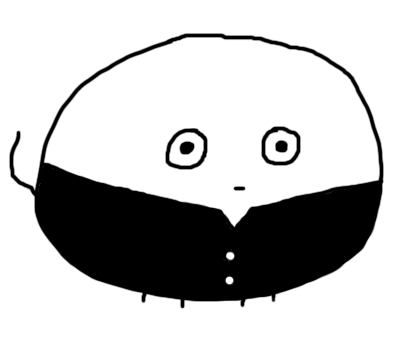
\includegraphics[width=0.9\textwidth]{img/noneccentricpianoprodigy}
\end{center}
\caption*{{\em ``Non-Eccentric Piano Prodigy'' Hamster}.}
\end{figure}
In a 2013 feature article
in {\em The New York Times Magazine} a {\em ``Non-Eccentric Piano Prodigy'' 
Hamster} named John Thomason atypically received extensive coverage---to the 
extent of 5839 words, of which 4794 were, however, focused on the question of 
``exactly
why'' the article's author has ``long harbored the strong
suspicion'' that the specific {\em ``Non-Eccentric Piano Prodigy'' Hamster}
named John Thomason is ``being non-eccentric on-purpose?'' and therefore,
from a certain ``second level'' perspective, actually way more eccentric
than the {\em ``Eccentric Piano Prodigy'' Hamster}, whose eccentricity is
conveyed ``directly, genetically, honestly, and without
irony---without,'' according to the article's author, Janice Mikaela,
``the questionably legitimate post/meta-artfulness that John Thomason has
subtly deployed in his life and work ever since, as far as my research shows, he
was born.'' The feature article included two full-page photographs
and---interspersed throughout---eight smaller photographs (these smaller
ones focused on her eyes, hands, forearms, mouth, forehead, and hair) of Janice
Mikaela, who was previously known primarily for her eccentric behavior at panel
discussions and ``elegantly outrageous'' ({\em Vogue}) hairstyle, instead of
portraits of the pianist, who also was not interviewed or contacted for the
article.

\vspace{2em}

\noindent
\textbf{Hunting Tips:} Approach the {\em ``Non-Eccentric Piano Prodigy''
Hamster} after a concert asking for its autograph---stunning it, as no one 
cares enough to want its autograph. Ask another question---any question---to 
further destabilize the {\em ``Non-Eccentric Piano Prodigy'' Hamster}'s 
perception of reality (that no one is interested in it) in order to cause 
cardiac arrest, effectively ending its life. Finally, at your leisure, place 
it in a plastic baggie. \\

\newpage

\noindent
\textbf{Cooking Tips:} Baste in a paste of olive oil, wakame, hijiki, tamari 
at a low heat, ``moving it around'' occasionally. Serve over a thick---but not
 too thick---bed of lettuce. Great with red wine, diluted carrot juice,
 or---surprisingly---almond milk.

\begin{sidewaystable}
\begin{center}
  \small
  \begin{tabular}{rl}
  \textbf{Average weight/height (record)} & .9 lbs/3.3" (1.6 lbs/3.9") \\
  \textbf{Average life expectancy (record)} & 18.4 years (36.9 years) \\
  \textbf{Favorite book(s)} & {\em The Mind of God} \\
  \textbf{Favorite band(s)} & anything by Chopin, Brahms \\
  \textbf{Favorite movie(s)} & {\em Eternal Sunshine}  \\
  \textbf{Favorite sexual position} & missionary \\
  \end{tabular}
\end{center}
\caption*{{\em``Non-Eccentric Piano Prodigy Hamster''} facts.}
\end{sidewaystable}


\end{document}

